\chapter{Implementation \& Testing}
Following from the analysis and design of the application, it is now possible to start implementing the features produced from investigating the requirements earlier in the project. As it was already stated that the project would be running under an FDD means, rather than having two sections (one for implementation and one for testing), this section will show each feature one-by-one. By following this scheme, the feature prioirty list will be utalised to ensure the more important features are done first, and that they fulfil their function before moving on. However, this should not hide the fact that issues are possible when implementing and any such issues could hamper further development. If this does occur, the issues and reasons will be explained, followed by what judgement was made to continue on with development of the application as a whole.

\section{FDD project approach}
As mentioned, the feature driven development methodolodgy will now shape the approach that is taken to create each feature. Although design has already been completed for all features, there are still elements to each iteration that should be outlined before proceeding. The best way to plan this is to give a brief list of steps that will be performed in each iteration. This is as follows:

\begin{enumerate}
\item Give a re-cap on the requirements of the feature
\item Provide a walkthrough of implementation (with code samples)
\item Show tests used (JSUnit, usability tests) and results
\item Describe and differences with the feature and original design
\item If there are any issues, describe and give explanations
\item Give a progress log on the item, and provide dates and length of completion for use in accordance with the Gantt chart originally constructed
\end{enumerate}

It should also be noted that once the duration of the time in the project for the implemtation and testing stage is complete, a burn down and progress report will be possible to generate and will be done so. This will give a good idea of exactly the status of the project (with a calculated percentage), to see how much work was done compared to estimates, and to find out how succesful the project was overall. 

\subsection{Iterative Implimentation}
Before the iterations begin, it should be mentioned that although the order of features to be implemented were decided in the analysis, in order to impliment any back end things and allow for proper testing (usability testing), some basic GUI must be created first. Becuase of this, this will be the first iteration, followed by creation of the JSON manoeuvres. Following these iterations, it will then be much easier to test future features created. Without a basic GUI and canvas, it will be impossible to see the effects created whilst adding features such as drawing flight paths or moving cameras. After these two moved features are complete, the prioritised list will run as planned initially.

\subsubsection{Feature 1- Create a basic GUI}
The first feature that was to be implemented was less of a feature but more a requirement so the other features could be then created. The GUI or front-end of the application is important to be created, otherwise testing future WebGL features will not be possible. The requirements of the front end were:

\begin{itemize}
\item A responsive front-end that is mobile compatible
\item Have hidden menus that can push in from the left
\item Have basic inputs such as the OLAN input, and menu options
\item Provide a help and about page that overlays the application web page
\end{itemize}

The first task that was performed to create this task was to create a minimulistic layout matching the wireframes designed in chapter 2 of this report. The first action performed was to get the latest Foundation \cite{foundation} css library file, and then to create a layout using the features from the library. The navigation was made using the 'navbar' markup, which helps stick the navbar to the top of the page, alongside automatically changing into a mobile pull down menu once the screen size reaches a certain amount. Then using other mark-ups provided by Foundation I was able to float the various navigation bar buttons to their respective sides. 

The most important part of the GUI which has now been implimented is the off-canvas feature menus. The code for this can be seen in section~\ref{code:canvas} of appendix C. The way that Foundation helps create this off cnvas option is by wrapping everything in one div, then seperating the menu and content in half. When a user then pushes the designated button with the wrapper id, the entirety of the wrapper is pushed to the right to display the menu and less of the content. The about and help pages were also added successfully, with the addition of another library called Modernizer. This library allowed for a clean effect to overlay the information on top of the webpage.

Once the basic HTML elements with relevent ID tags were added to the index page of the application, it was then possible to add some custom style to the page. As mentioned in the design stage, it was possible to download Foundation modified with the colour scheme designed for the application. Changing backgrounds to black and text to white was very easy, and then added to the site. The colour and design of the page can be seen below in figure~\ref{fig:newgui}.

\begin{figure}[h]
  \centering
      %\includegraphics[width=1\textwidth]{images/newgui.png}
  \caption{Screenshot of GUI created with Foundation, JQyery and HTML markup.}
  \label{fig:mod}
\end{figure}

As planned, Sass was used to style specific elements of the page, such as the width of the OLAN input box, and to change text placement on the help and about pages. Setting up the Sass with Koala was easy, and upon each save of the file, CSS was compiled. 

One final mention goes to the creation of the WebGL canvas. To create the basic canvas, only a few lines of JavaScript was needed. To create it, a renderer was created using  the 'THREE.WebGLRenderer' object. Becuase this is early in the implementation stage, it was created without RequireJS as the archetcure is only one JS file. Once the object is created, JQuery appends the '.domElement' of this object to the container div created in the basic HTML. For future features, the WebGLRenderer object with be where any objects such as flight paths are added to.

As for testing this feature, becuase very little JavaScript was required to be coded here, usability testing was the only way to check for the completion of what was required. The test results can be found in Appendix D under section~\ref{test:canvas}. Overall, this feature has been made to 100\% of the requirements laid out, and matches the deisgn very well. Therefore, the progress tracker for this feature can be shown as:

\begin{table}[h]
\begin{tabular}{|l|l|l|l|p{7cm}|}
\hline
\textbf{Start} & \textbf{End} & \textbf{Duration} & \textbf{Progress} & \textbf{Comments}                                                                                                     \\ \hline
09-03-2015     & 10-03-2015   & 2 Days            & 100\%             & Complete, though once new features are under way, RequireJS will be utalised and the WebGL Canvas code will be moved. \\ \hline
11-03-2015     & 11-03-2015   & 1 Day            & 100\%             & Testing complete, usability table created and tested on mobile and desktop devices.\\ \hline
\end{tabular}
\end{table}

\textbf{Feature overall progress: 100\%}

\subsubsection{Feature 2- Convert OLAN and Aresti to JSON form}
The second feature, which was of high importance to the rest of the application was to create OLAN interpreted JSON which would give instrctions on how to construct each manoeuvre. Becuase this was quite thoughroughly planned and then designed how each instruction was going to broken down, the time designated for this task felt generous. Simply using the template created in the design, it was possible to fill in each instrction part by part through each OLAN manoeuvre. An example of some instructions can be seen in Appendix C in section~\ref{code:jsonmoves}.

The only time consuming part of this feature was the shear amount of different manoeuvres that had to be converted. For this reason, not every OLAN letter was created. The reason for this is becuase some moves are possible to be created from others, so further in development, more will be possible to be added. 

To support this feature, more JavaScript code had to be added to allow the JSON to be read into an object to begin drawing moves onto the canvas. Becuase the code would be in a different module to the WebGL canvas that was created in the previous feature, RequireJS now had to be added to the source code. To do this, the RequireJS library was added and initiated in the HTML page of the application as shown here in Appendix C section~\ref{code:requireJS}. Then a new module was created, named 'Dataparser' as designated in the design. The method for converting the JSON can also be found in the data parser module shown again in the appendix under section~\ref{code:jsonmovesJS}.

Once the coding and converting to JSON was complete, testing the code that performed the conversion to an object was required. By using JSUnit, it was possible to call the method that was created to instantiate the manoeuvres array, and pass in some raw JSON string, then compare to what the result should be. The JSUnit code can be found in appendix D, section~\ref{test:jsonmvoes}.

Like the last feature, no changes from the original design were performed, resulting in a good standing of time compared to the Gantt chart for the project. The feature progress can be expressed as percentages and final comments added again.

\begin{table}[h]
\begin{tabular}{|l|l|l|l|p{7cm}|}
\hline
\textbf{Start} & \textbf{End} & \textbf{Duration} & \textbf{Progress} & \textbf{Comments}                                                                                                     \\ \hline
12-03-2015     & 16-03-2015   & 5 Days            & 80\%             & JSON created to represent most manoeuvres, for that reason it is not an exact 100\& progress. JavaScript code and RequirejS functionality added to support the rest of the application. \\ \hline
17-03-2015     & 18-03-2015   & 2 Days            & 100\%             & JSUnit tests created and passed successfully, showing JSON matches up with manouvre array object.\\ \hline
\end{tabular}
\end{table}

\textbf{Feature overall progress: 90\%}

\subsubsection{Feature 3- Creating a scene with terrain and lighting}
The third feature, which is another to be brought forward ahead of flight path creation is the terrain and lighting effects. The reason for creating this before the OLAN construction is the same as creating the canvas, becuase without an area to see where the paths are drawn onto, the effects of that feature will be hard to test if it is working. Especially terrain, where the need for this is to see where the X axis of 0 will be. Without this, when implementing checks such as if the path would hit the ground would be harder to test. Again, the three.js library was of great use here, especially with built in methods to allow for lighting to be added.

In order to have started this feature, another module was added to the archetecture named 'TerrainHandler', which was where both lighting and ground was to then have their methods of adding to the canvas. This feature was found to be the shortest of the features, as it only required two simple methods. Rather than passing the renderer canvas object to this module to add the ground and lighting, it was decided to simply make both methods like factories to return the ground and lighting objects to where they were called from. In the case of where this module was called from, the main class where the canvas was created seemed the best place to call each method, as everything to do with setting up the scene could remain together and be easily understood or developed further.

As for testing, by keeping the terrain and lighting in their own module also helped towards testing the new methods. Two very simple tests were made using JSUnit to check the returns of each method, and both were added to the Jasmine instructions under each Github commit through the Travis builds. As with other tests, the test cases can be found in the appendices under appendix D section~\ref{test:lights}. This feature was fairly straight forward to implement and test with help from the three.js documentation site, therefore teh feature was done in less time than originally planned.

\begin{table}[h]
\begin{tabular}{|l|l|l|l|p{7cm}|}
\hline
\textbf{Start} & \textbf{End} & \textbf{Duration} & \textbf{Progress} & \textbf{Comments}                                                                                                     \\ \hline
19-03-2015     & 20-03-2015   & 1 Day            & 100\%             &  Completed module for terrain and lighting, linked up to main module.\\ \hline
20-03-2015     & 20-03-2015   & 1 Day            & 100\%             &  Two JSUnit tests created, and passing successfully.\\ \hline
\end{tabular}
\end{table}

\textbf{Feature overall progress: 100\%}

\subsubsection{Feature 4- Cameras}
The final predessing feature before the creation of OLAN paths that was decided should be ready were the various cameras that will look around the canvas. The initial requirements for cameras was to have two different views: one for navigating around the canvas, and the other for being onboard the flight path. At this stage of the project, creating the second was only possible to a certain extent, becuase without the construction of the paths yet, getting the location of where the onboard camera should be is not possible. Therefore, for this requirement both cameras were created, with the exception of the onboard camera where functionality is currently restricted. 

To start, another module was created for the 'CameraController'. Becuase it was best to keep the cameras completely seperated from other parts of the application to reduce decoupling, both camera objects were stored in this module and provided get and set methods for calls from other modules. An inititiator method was created for use from the main module, to create both camera objects at start up. Both these objects were again availible from the three.js library as 'THREE.PerspectiveCamera'. Then by passing the module around to any other modules, it will then be possible to update and retreive each camera object again. Alongside the camera creation, a controller for changing the angle of view, zoom and co-ordiantes was created as another module. 

This module, which has been called 'CanvasController' as designed in the module diagram, adds event listeners for dragging the mouse around the canvas, keyboard presses to move up and down, and scroll for zooming. Then by getting the new updated values of view-point angles, these are passed back to the camera controller which updates the values of each camera. By repeating this in a render loop in the main module, the updating of cameras is done several times a second, to make movements appear fluid. To help this, the code was refeactored several times to ensure that the amount of work done by the browser is as little as possible on each loop of the animation.

As for testing, alike the first feature where usability testing was the primary and sole means of checking the implementation fulfills the feature, JSUnit testing was not used. Usability testing was found the best option here, and results can be found in appendix D section~\ref{test:cameras}. During testing, it was found that there was an issue that when rotating the camera around the canvas, it seemed to always rotate around the point (0,0,0). This meant that navigating the canvas was slightly harder than it should have been. This was fixed though, by simply moving the camera rather than the scene in the canvas. As for the camera that was designed to be as on board view, a model airplane was added to represent the camera so it could be seen on the canvas. Although it does not move yet, the plane loads up at the start of the application and can be placed anywhere on the scene. You can see the plan on the canvas at point (0,0,0) below in figure~\ref{fig:plane}. The plane model is constrcuted from a JSON file from a page on the web with thousands of free models.

\clearpage

\begin{figure}[h!]
  \centering
      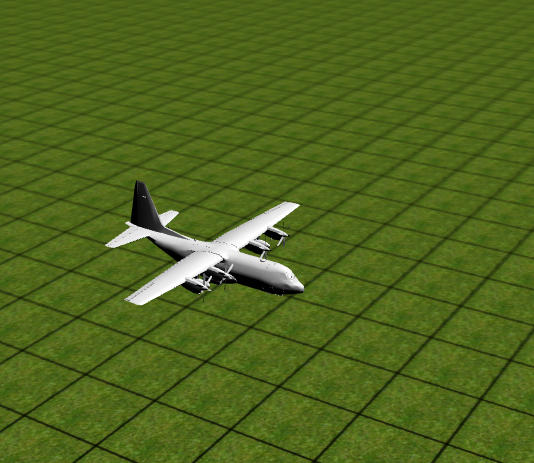
\includegraphics[width=0.6\textwidth]{images/plane.png}
  \caption{Model of plane loaded up using JSON and three.js object loader. This plane will represent the onboard camera, and fill be the object that will be assigned locations along an OLAN path to show flying the flight plans entered by users.}
  \label{fig:plane}
\end{figure}

The progress of the task is shown below. This feature was done exactly to its requirements in the design, and the modulation of code is still being followed.

\begin{table}[h]
\begin{tabular}{|l|l|l|l|p{7cm}|}
\hline
\textbf{Start} & \textbf{End} & \textbf{Duration} & \textbf{Progress} & \textbf{Comments}                                                                                                     \\ \hline
21-03-2015     & 23-03-2015   & 3 Days            & 100\%             &  Both cameras now usable, with constructer methods, and update methods. On board camera ready but not linkable to rest of application until animation of flight paths is ready.\\ \hline
24-03-2015     & 24-03-2015   & 1 Day            & 100\%             &  Usability tests complete, one change made to code following a failed test. \\ \hline
\end{tabular}
\end{table}

\textbf{Feature overall progress: 100\%}

\subsubsection{Feature 5- Construction of 3D paths from OLAN}
The most important feature, drawing shapes onto the canvas using the instrctions read in from JSON files was next to be implemented. The main requirement here was to draw smooth shapes that match the Aresti shapes as accuratly as possible, also bearing in mind that they should be linkable.

\section{Final status and progress}
\subsection{Implementation and testing review}
%The implementation should look at any issues you encountered as you tried to implement your design. During the work, you might have found that elements of your design were unnecessary or overly complex; perhaps third party libraries were available that simplified some of the functions that you intended to implement. If things were easier in some areas, then how did you adapt your project to take account of your findings?It is more likely that things were more complex than you first thought. In particular, were there any problems or difficulties that you found during implementation that you had to address? Did such problems simply delay you or were they more significant? You can conclude this section by reviewing the end of the implementation stage against the planned requirements. 

%Detailed descriptions of every test case are definitely not what is required here. What is important is to show that you adopted a sensible strategy that was, in principle, capable of testing the system adequately even if you did not have the time to test the system fully.Have you tested your system on �real users�? For example, if your system is supposed to solve a problem for a business, then it would be appropriate to present your approach to involve the users in the testing process and to record the results that you obtained. Depending on the level of detail, it is likely that you would put any detailed results in an appendix.The following sections indicate some areas you might include. Other sections may be more appropriate to your project. 